\section{Projektbeskrivelse}

\subsection{Indledning}
Der er blevet tildelt et panorerings- og tilt-system, hvor tilt rammen er monteret på pan rammen. Se Figur \ref{fig:Opstilling}.\\
Et sådan system bruges til observatorier, lysudstyr, overvågningskameraer samt mange andre applikationer.\\
Til følgende beskrivelse af systemet er der ønsket en valgfri meningsfyldt applikation.\\
For at pan-rammen ikke ødelægger ledningerne til tilt-rammen, er der tilføjet en stopklods, der forhindre pan-rammen i at gå udover denne begrænsning. Tilt-rammen er ubegrænset i dens bevægelser.\\
Til rammerne er der tilføjet to EMG30\cite{emg30Data} motorer, en på hhv. pan- og tilt-rammerne.\\
På rammerne er også monteret 2 hall sensorer med tilhørende magneter. Til brug ved nulstilling af systemet.

\begin{figure}[H]
	\begin{center}
		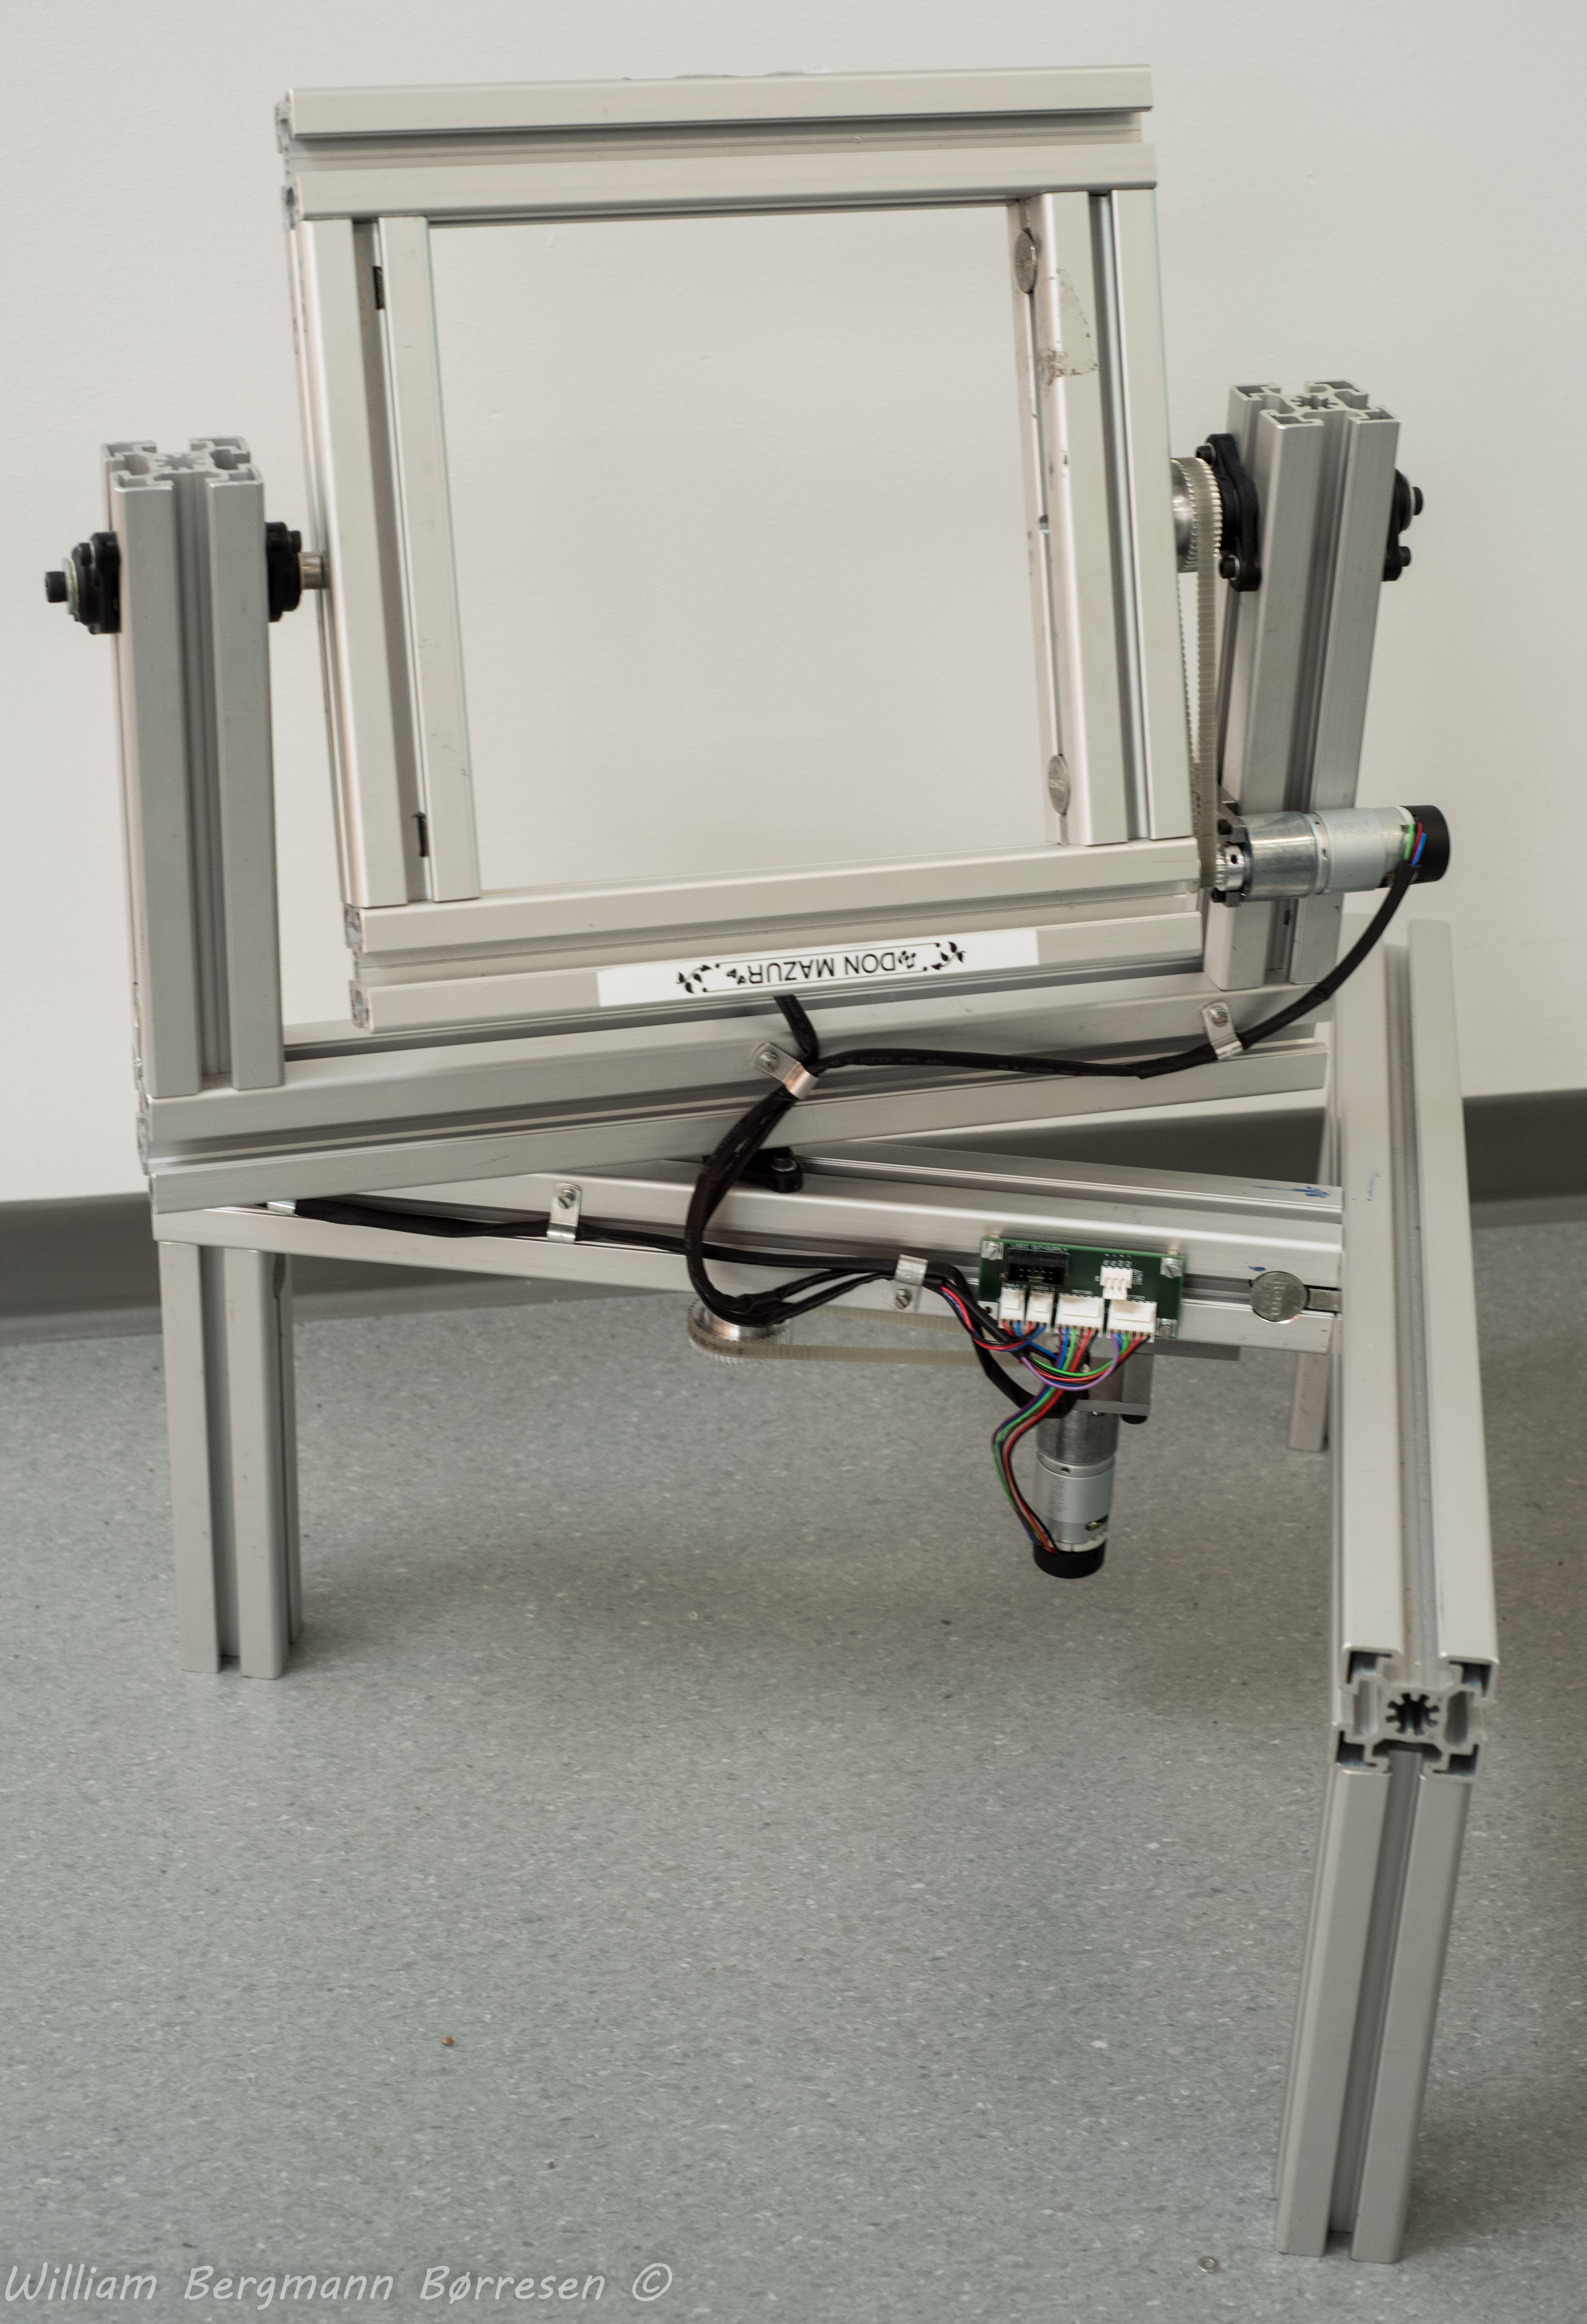
\includegraphics[scale=0.15]{Billeder/opstilling.jpg}
		\caption{Opstilling af panorerings- og tilt-systemet med motorer og hall sensorer monteret.}
		\label{fig:Opstilling}
	\end{center}
\end{figure}

\subsection{Problemformulering}

Vil det være muligt at lave et system som er præcist nok til at tage billeder af bestemte stjerner, månen, solen og/eller satellitter?\\
Hvilken form for controller vil være mest optimal til et præcist, og ikke nødvendigvis hurtigt, system?\\
Hvordan kan et pan/tilt-system styres med koordinater som input?\\
Hvordan kan det sikres at systemet ikke går udenfor sine mekaniske begrænser under anvendelse?

\subsection{Kravspecifikation}

Hvis pan/tilt-systemet f.eks. skal pege på den internationale rumstation, som bevæger sig rundt i en afstand omkring 400 km væk fra jorden, og peger en enkelt grad forkert, vil systemet næsten pege 7 km ved siden af. Derfor er det vigtigeste krav i dette project, at vi ingen steady state fejl har ved forstyrrelser, der kan opstå under normal drift.

\subsubsection{Arbejds- og fagområder}
Pan/Tilt-projektet bliver udarbejdet for at give en bredere og bedre forståelse for 4. semesters fagene. På baggrund af dette er der valgt nogle arbejds- og fag-områder som sørger for at projektet kommer til at have indhold fra hvert fag.\\
4. semester fagene består af:
\begin{itemize}[noitemsep]
	\item Computer Operativ Systemer (COS)
	\item Embedded Programmering (EMP)
	\item Reguleringsteknik (REG)
	\item Digital Programmerbar Elektronik (DIG)
\end{itemize}

\subsubsection{Obligatoriske Krav}

\begin{itemize}[noitemsep]
	\item COS/EMP
	\begin{itemize}[noitemsep]
		\item Task-baseret operativsystem med schedulering
		\item SPI-Kommunikation mellem microcontroller og FPGA
	\end{itemize}
	\item REG
	\begin{itemize}[noitemsep]
		\item Systemanalyse og modellering af systemets enkelte elementer
		\item Closed-loop controller
	\end{itemize}
	\item DIG
	\begin{itemize}[noitemsep]
		\item SPI-protokol til FPGA
		\item PWM driver til FPGA
		\item Motor position skal bestemmes af FPGA
	\end{itemize}
\end{itemize}

\subsubsection{Primære opgaver}

Som krav til systemet skal det kunne tage et input i form af et horisontalt koordinatsæt, som systemet så omsætter til sfæriske koordinatsæt, en vinkel for pan og en vinkel for tilt. Yderligere er det nødvendigt at systemet kan tage manuelt indtastning af koordinatsæt som alternativt input.

Som en del af COS/EMP faget sættes der som krav, at systemet skal kunne give feedback gennem LCD komponenten i form af den nuværende position i horisontale koordinater. Der skal kunne tages input fra knapper på EMP board'et, og en UART-forbindelse, med tilsvarende UART-protokol, skal kunne forbinde board'et med en computer.

Der skal laves en PID-controller, som beskrevet i REG, der er foruden både XXXX overshoot og steady state fejl. Yderligere skal systemet kunne bevæge sig 180 grader og stoppe på under fem sekunder, med en usikkerhed på højest én grad.

Samtidig skal der laves et stykke funktionelt, digitalt programmeret, elektronik, i form af et FPGA board, der skal fungerer som en ``slave'' for microcontrolleren, og give denne information om positionen af systemet samt benytte denne til at sætte hastighed og retning på motorerne. Microcontrolleren skal også fungere som en sikkerhed, der endegyldigt sikrer at der ikke kan ske uheld, ved at systemet kører ud over sine mekaniske begrænsninger.

\subsubsection{Sekundære opgaver}

De sekundære krav til systemet som helhed, og tilsvarende applikation, er at dette kan udregne baner for himmellegemer og hente live oplysninger fra internettet om legemers positioner. Yderligere skal systemet kunne styres ved brug af en direkte kontrol af position uden brug af koordinater, og et kamera skal monteres i pan-tilt-systemet. Endeligt skal der være mulighed for at et bluetooth modul kan benyttes til UART-kommunikation.

Til COS/EMP fagene er det sekundære krav at systemet kan overvåges gennem UART, således at der kan holdes styr på performance af controlleren og hvorvidt den ønskede position er overholdt, således at der kan tages automatiske billeder.

Det sekundære krav til REG er at PID-controlleren er i stand til at selvkalibrere til et givent system.

Til DIG er det sekundære krav at denne er i stand til at omregne systemets koordinater til grader.